\section{Methodology validation}
In this chapter, the proposed methodology will be validated, developing a map three-dimensional and a digital elevation model with the Agisoft Photoscan.
\subsection{Mission planning}
\textbf{Weather condition checks}\newline
The day the mission was executed the weather conditions are displayed in table \ref{Table:Weather}
\begin{table}[H]
\centering
\begin{tabular}{|c|c|}
\hline
\multicolumn{2}{|c|}{Weather conditions.} \\ \hline
Wind average {[}m/s{]}         & 7        \\ \hline
Wind gusts {[}m/s{]}           & 12       \\ \hline
Wind direction (degrees)       & 180      \\ \hline
Temperature {[}c{]}            & -1       \\ \hline
Precipitation {[}mm{]}         & 0        \\ \hline
\end{tabular}
\caption{Weather condition for the mission}
\label{Table:Weather}
\end{table}
\textbf{Surveying area, Hardware used and Requirement definition}\newline
\textit{Study area}

All the flight test were carried out in the Odense model airfield, situated 20km north of city. The field has an approximated are of around 74400 $m^2$. figure \ref{fig:Airfield} shows a satellite image of the airfield
\begin{figure}[H]
\centering
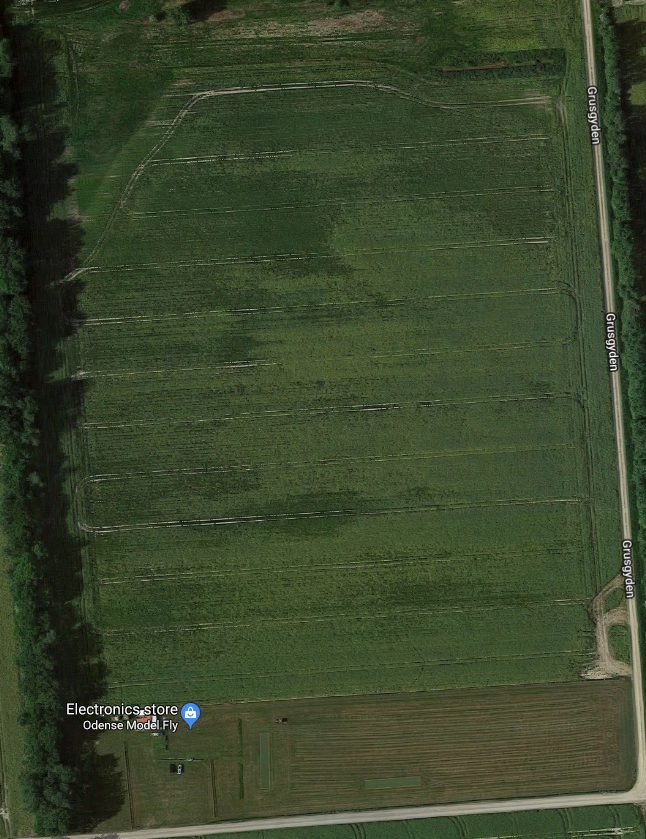
\includegraphics[width=6cm,height=6cm,keepaspectratio]{imagenes/Satellite.png}
\caption{Satellite view of Odense model airfield}
\label{fig:Airfield}
\end{figure}

There are two different study area in the field one two the left (Field A), the other to the right (Field B) of the field. The figure \ref{fig:Study area} shows two study areas delimited by a blue line,the table \ref{table: Area_char} presents details of the study areas.
\begin{figure}[H]
\centering
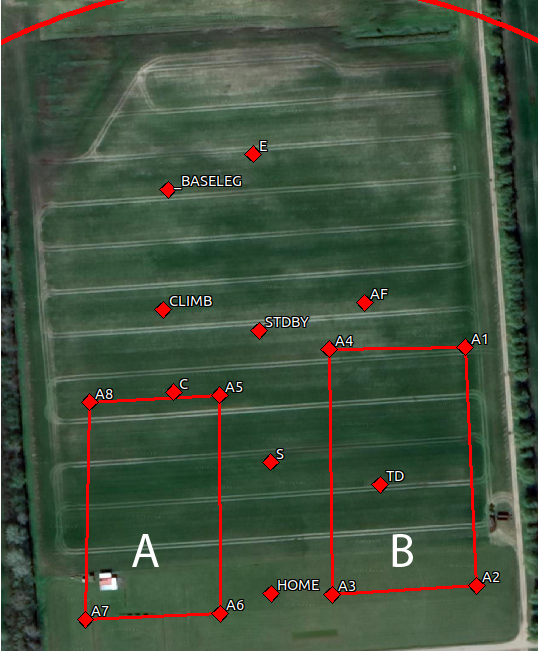
\includegraphics[width=6cm,height=6cm,keepaspectratio]{imagenes/Study_Area.png}
\caption{Study area for the project}
\label{fig:Study area}
\end{figure}

\begin{table}[H]
\centering
\begin{tabular}{|c|c|c|c|c|}
\hline
Area & Length X (m) & Length Y (m) & Area ($m^2$) & Elevation (MAMSL) \\ \hline
A     & 74           & 113         &  8362     & 0                 \\ \hline
B     & 75           & 105          & 7875      & 0                 \\ \hline
\end{tabular}
\caption{Study area characteristics}
\label{table: Area_char}
\end{table}
The area where the mission will be executed was a row of trees on both sides of the field; this condition generates two mission limitations: The task should be performed with a minimum flying altitude of 20 m to avoid a collision with the trees, and the lading will be conducted with a crosswind Figure \ref{fig:ARboles}
\begin{figure}[H]
\centering
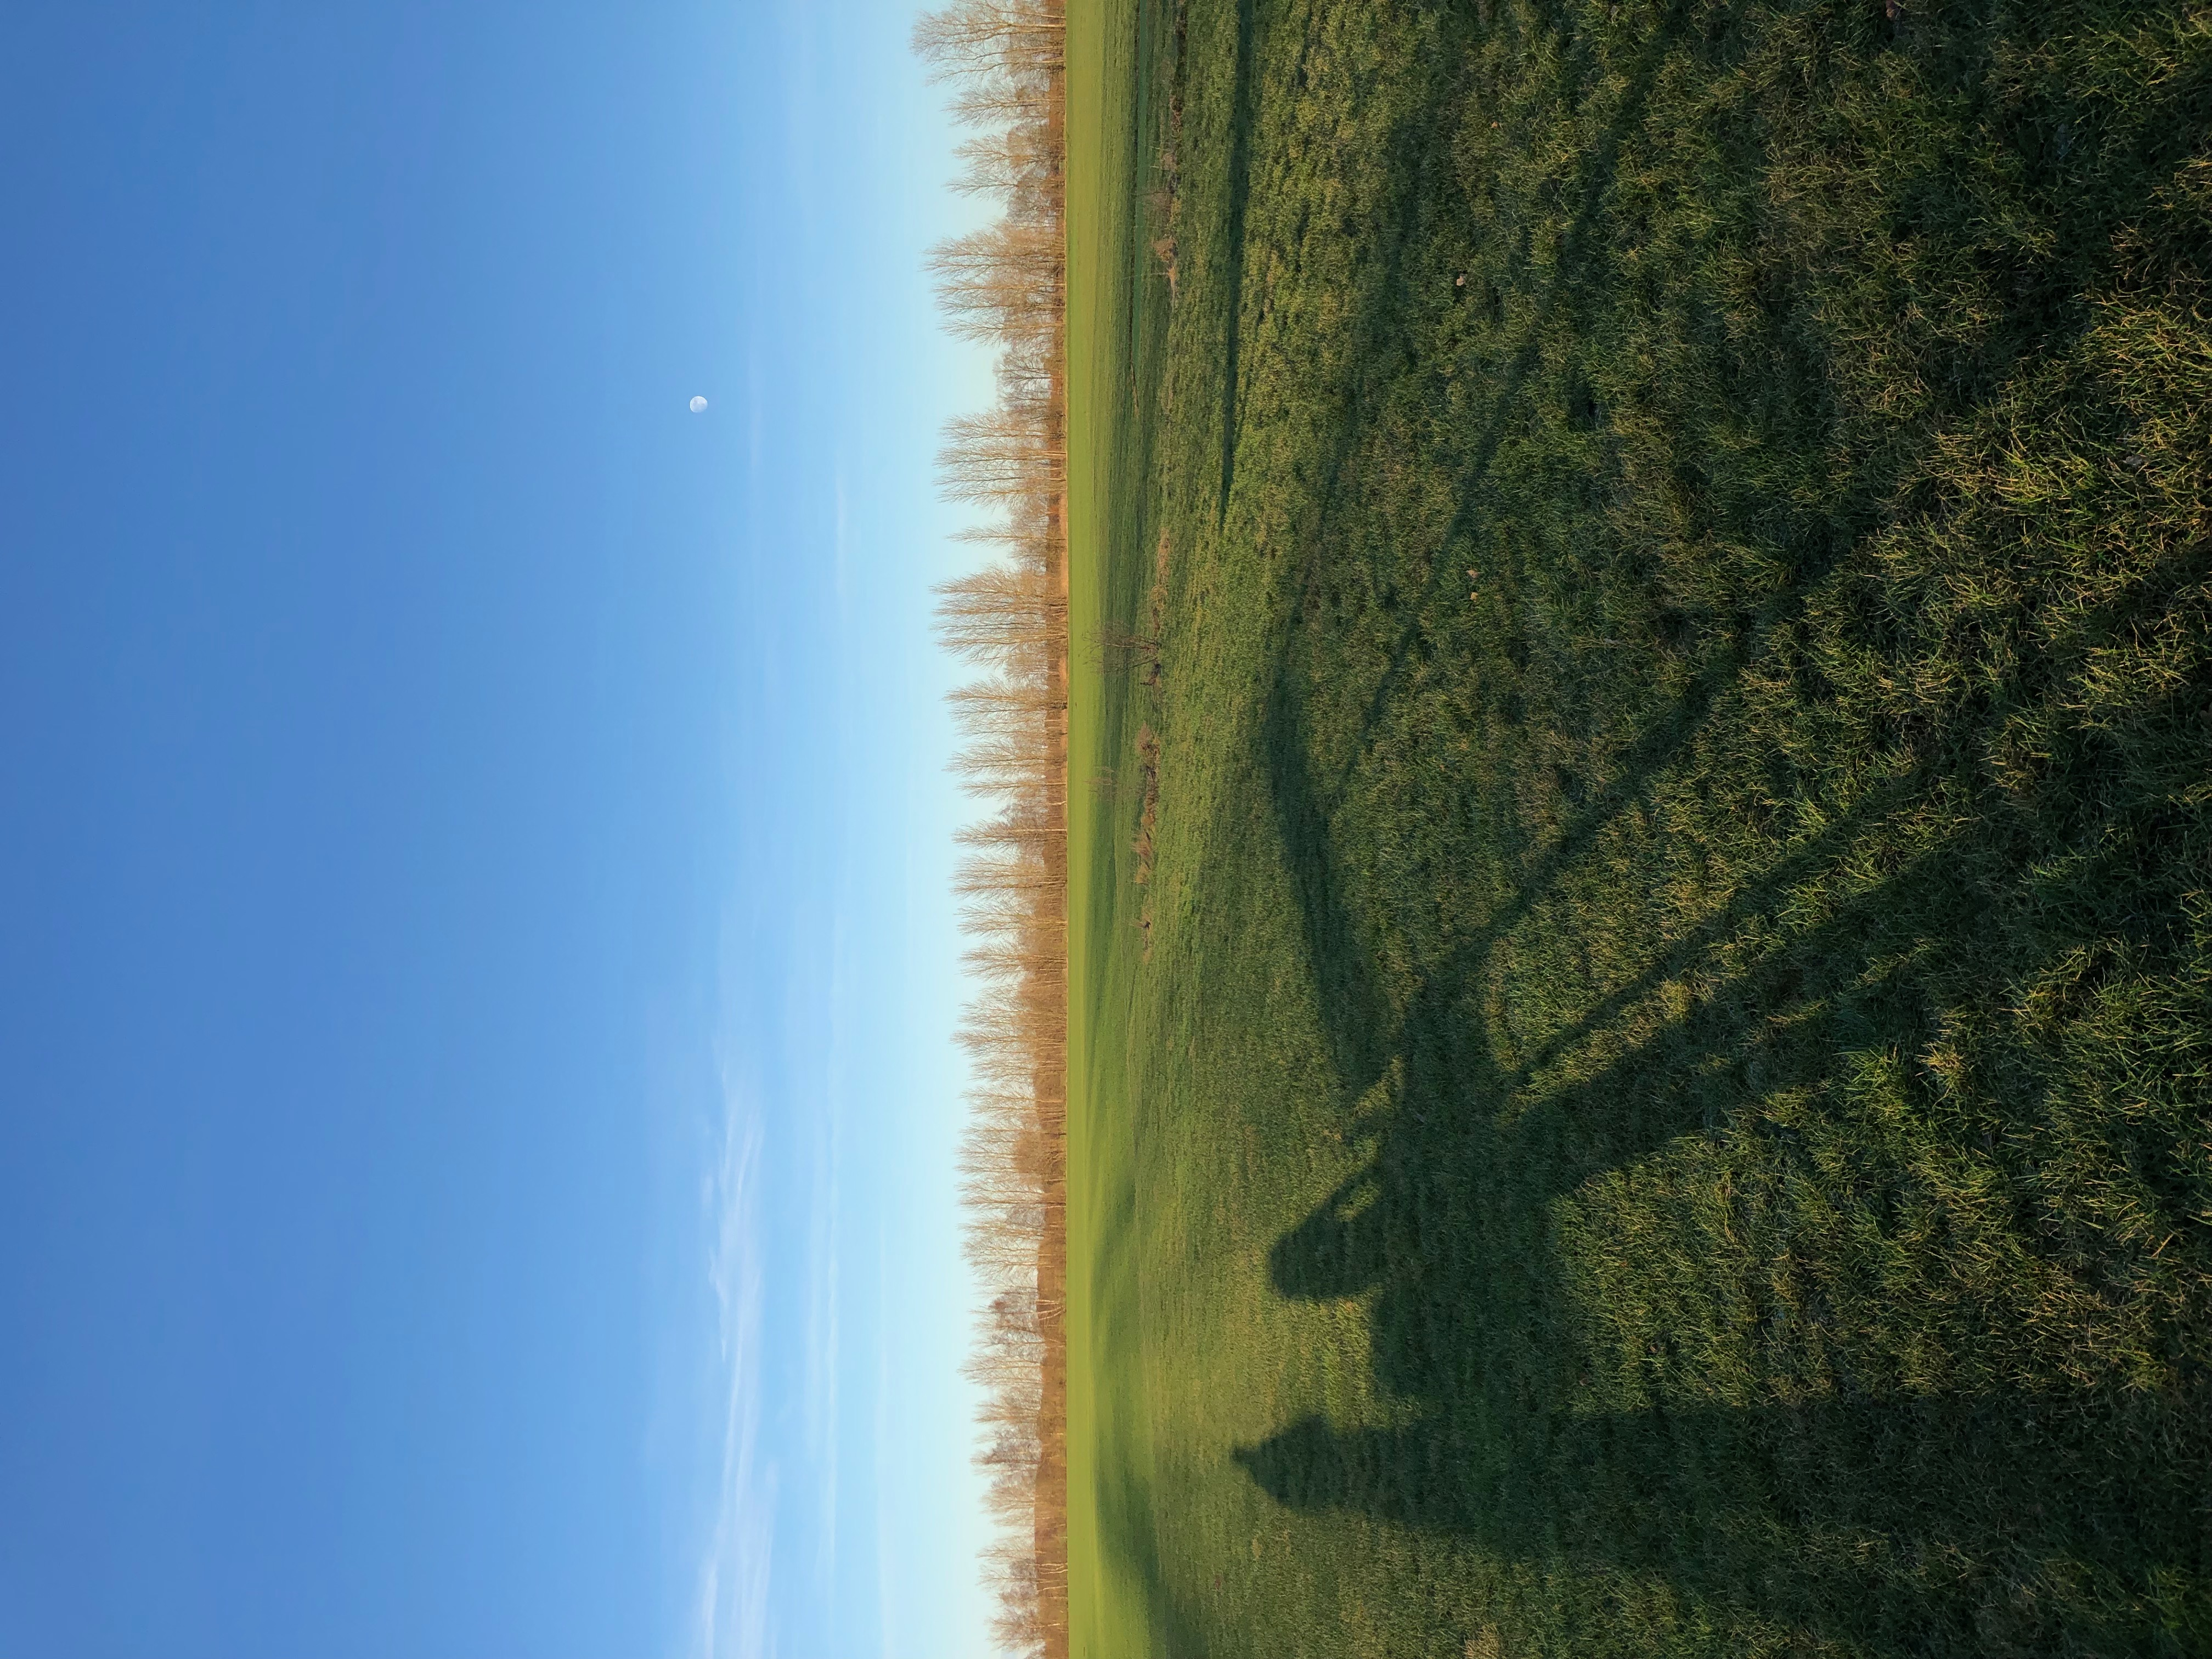
\includegraphics[width=8cm,height=8cm,keepaspectratio,angle=-90]{imagenes/IMG_1122.JPG}
\caption{Trees on the field sides}
\label{fig:ARboles}
\end{figure}
\textbf{Hardware description}\newline
\textit{Ground segment:}
In this section can be found a description of the hardware used to preform the studies.
The ground segment hardware is described in table \ref{Table:Ground_Hardware}
\begin{table}[H]
\centering
\begin{tabular}{|c|c|}
\hline
Hardware             & Description                            \\ \hline
Ground Computer      & Macbook Pro running Ubuntu 18.04.1 LTS \\ \hline
Ground software      & Paparazzi UAS                          \\ \hline
Ground side data link & Xbee Pro 2.4GHz, 18 dBm (63mW)         \\ \hline
Ground side safe link  & Futaba T-FHSS 14 Channels               \\ \hline
\end{tabular}
\caption{Ground segment hardware}
\label{Table:Ground_Hardware}
\end{table}


\textit{Data link:}
Both up and down link use \textit{XBee Pro S1}. the performance specification can be found in table \ref{Table:XBee}
\begin{table}[H]
\centering
\begin{tabular}{|c|c|}
\hline
Specification           & Description   \\ \hline
Range                    & 1600 m        \\ \hline
transmit power output    & 63mW (18 dBm) \\ \hline
RF data rate             & 250000 b/s    \\ \hline
Receiver sensitivity     & 100 dBm       \\ \hline
Operating frequency band & 2.4GHz ISM    \\ \hline
\end{tabular}
\caption{Data link segment hardware specification}
\label{Table:XBee}
\end{table}

\textit{Air segment:} Table \ref{Table:Air_Segment} details the air segment specification 
\begin{table}[H]
\centering
\begin{tabular}{|c|c|}
\hline
Hardware                             & Description                                                                                                                                                          \\ \hline
Airplane                             & Opterra 2m                                                                                                                                                           \\ \hline
Autopilot                            & \multirow{3}{*}{ENAC Apogee autopilot with Paparazzi UAV}                                                                                                          \\ \cline{1-1}
IMU                                  &                                                                                                                                                                      \\ \cline{1-1}
\multicolumn{1}{|l|}{Altitud sensor} &                                                                                                                                                                      \\ \hline
GPS Receiver                         & NEO-M8T GPS + Magnetometer (Error: X,Y +- 4m, Z 4m)                                                                                                                                          \\ \hline
Data link modem                      & XBee Pro S1                                                                                                                                                          \\ \hline
RC reveicer                          & Futaba FASST                                                                                                                                                         \\ \hline
Servos                               & 2x 90 degree servos                                                                                                                                                  \\ \hline
Propultion type                      & 1300 Kv brushless motor with a 40A ESC                                                                                                                               \\ \hline
Batteries                            & 3 cell 3300mAh LiPo                                                                                                                                                  \\ \hline
Paylod                               & \begin{tabular}[c]{@{}c@{}}JeVois smart camera:\\ Focal length: 4.85mm\\ Resolution: 1280x1024\\ Sensor area: 4.13mmx3.28mm\\ Pixel size: 3.25$\mu$mx3.25$\mu$m\end{tabular} \\ \hline
\end{tabular}
\caption{Air segment hardware description}
\label{Table:Air_Segment}
\end{table}
\begin{figure}[H]
\centering
\includegraphics[width=10cm,height=10cm,keepaspectratio]{imagenes/UASSystem.JPG}
\caption{UAS system from left to right: Ground segment(Computer), Safe link (Futtaba transmitter), Air bone segment (Opterra 2m)}
\label{fig:UASSystem}
\end{figure}


\textbf{Theoretical computations}

The mission consists of surveying study area B with a 0-degree angle (South to North), and area A with a 180-degree angle (North-South). Using the equation from the Flight planning chapter with the parameters of tables. It is possible to compute the following (Front overlap and side overlap for both missions are 80\% , and GSD of 3.5 cm/pixel). Table \ref{Table: Valores} show the computed values:

\begin{table}[H]
\centering
\begin{tabular}{|c|c|c|}
\hline
Parameter                 & Field A & Field B \\ \hline
Space Between lines       & 9 m     & 9 m     \\ \hline
Distance between photos  & 7.2 m   & 7.2m    \\ \hline
Number of photos per line & 19      & 16      \\ \hline
Number of lines           & 9       & 8       \\ \hline
Flight altitude            & 50      & 50      \\ \hline
\end{tabular}
\caption{Value computation for flight planning}
\label{Table: Valores}
\end{table}
\textbf{Camera adjustment}\newline
A python program controls JeVois camera, the only setting that can be changed is the resolution of the image. In these study the resolution is 1280 x 1024 pixel, autofocus is turned off, due to the lack of shutter in the camera it is not possible to control the shutter speeds.

\footnote{In this study, the control point and landmark placement is not executed due to lack of proper equipment} 
\textbf{Flight path and mission simulation}\newline
The simulation of the mission is executed on the Paparazzi Ground Control Station (GCS). Compiling the mission code in NPS mode, it is possible to estimate the plane behavior and path. Figure \ref{fig:bsim} shows the simulation of Field B surveying mission.
\begin{figure}[H]
\centering
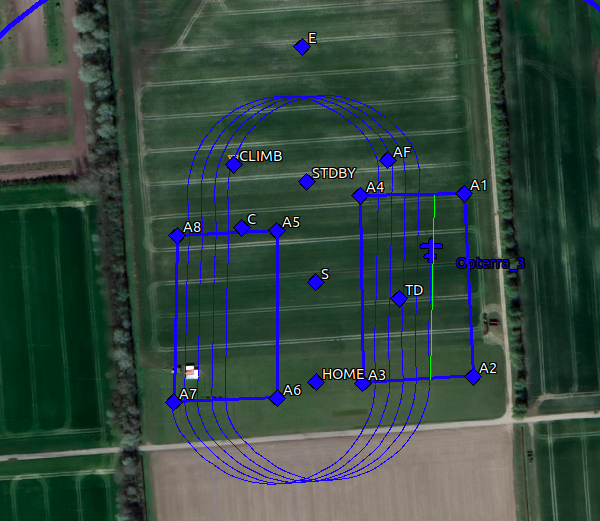
\includegraphics[width=10cm,height=10cm,keepaspectratio]{imagenes/SimBField.png}
\caption{B field surveying mission simulation}
\label{fig:bsim}
\end{figure}
The result of the simulation are displayed in table \ref{Table:SimResult}
\begin{table}[H]
\centering
\begin{tabular}{|c|c|c|c|}
\hline
Surveying Field & Number of photos & Number of strips & Execution time \\ \hline
A               & 125              & 8                & 7:10           \\ \hline
B               & 146              & 9                & 7:30           \\ \hline
\end{tabular}
\caption{Result of surveying mission simulation}
\label{Table:SimResult}
\end{table}
\subsection{System integration}
As mention before the payload for this mission is a JeVois smart camera. JeVois smart camera is capable of compiling and executing python and C++ programs. The camera is interfaced with the Apogee autopilot using the UART port and run on a python program.
 When the UAV is in the correct position, the autopilot sends a command to the camera to take a picture, also in this message the GPS position and attitude is sent to be saved in a data log. 

A 3D printed base was designed to be able to fix the camera to the UAV frame; it was necessary to cut two rails in the structure to slide the base in and take advantage of the existing mount. Figure n shows the 3D base. Figure \ref{fig:base} shows the JeVois mounted on the base.
\begin{figure}[H]
\centering
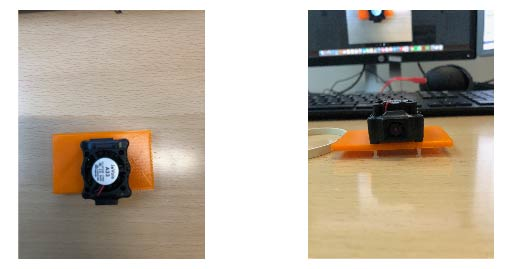
\includegraphics[width=10cm,height=10cm,keepaspectratio]{imagenes/Base.jpg}
\caption{JeVois camera with the 3D printed base}
\label{fig:base}
\end{figure}

This section presents an analysis of the data gathered on the surveying test mission executed on the Odense model airfield
\subsection{Mission execution}
This subsection presents an analysis emphasizing on the study of flight precision characteristics such as flight height, flight path, side, and front overlap. 
\subsubsection{Flight path}
Using the data logging capabilities of the Apogee, its possible to reconstruct the path traveled by the UAV.
Figure \ref{fig:SimVReal} shows a side by side comparison of the simulation and the real path flown by the UAV. The deviation on the flight its caused by the wind. The effect of the wind on the aircraft capability to follow the design path can have a significant impact on the success of the mission, especially since the fixed-wing UAV cannot hover or fly backward. 
\begin{figure}[H]
\centering
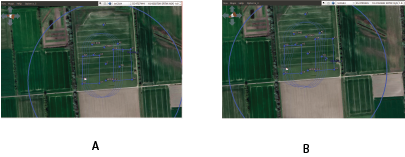
\includegraphics[width=14cm,height=14cm,keepaspectratio]{imagenes/SimVsreallity.png}
\caption{ A: Simulation of surveying mission. B: Surveying mission execution}
\label{fig:SimVReal}
\end{figure}
Using the geolocation of each picture is possible to recreate the UAV path. Figure \ref{fig:FielB} shows a line plot of the position of each photo.
\begin{figure}[H]
\centering
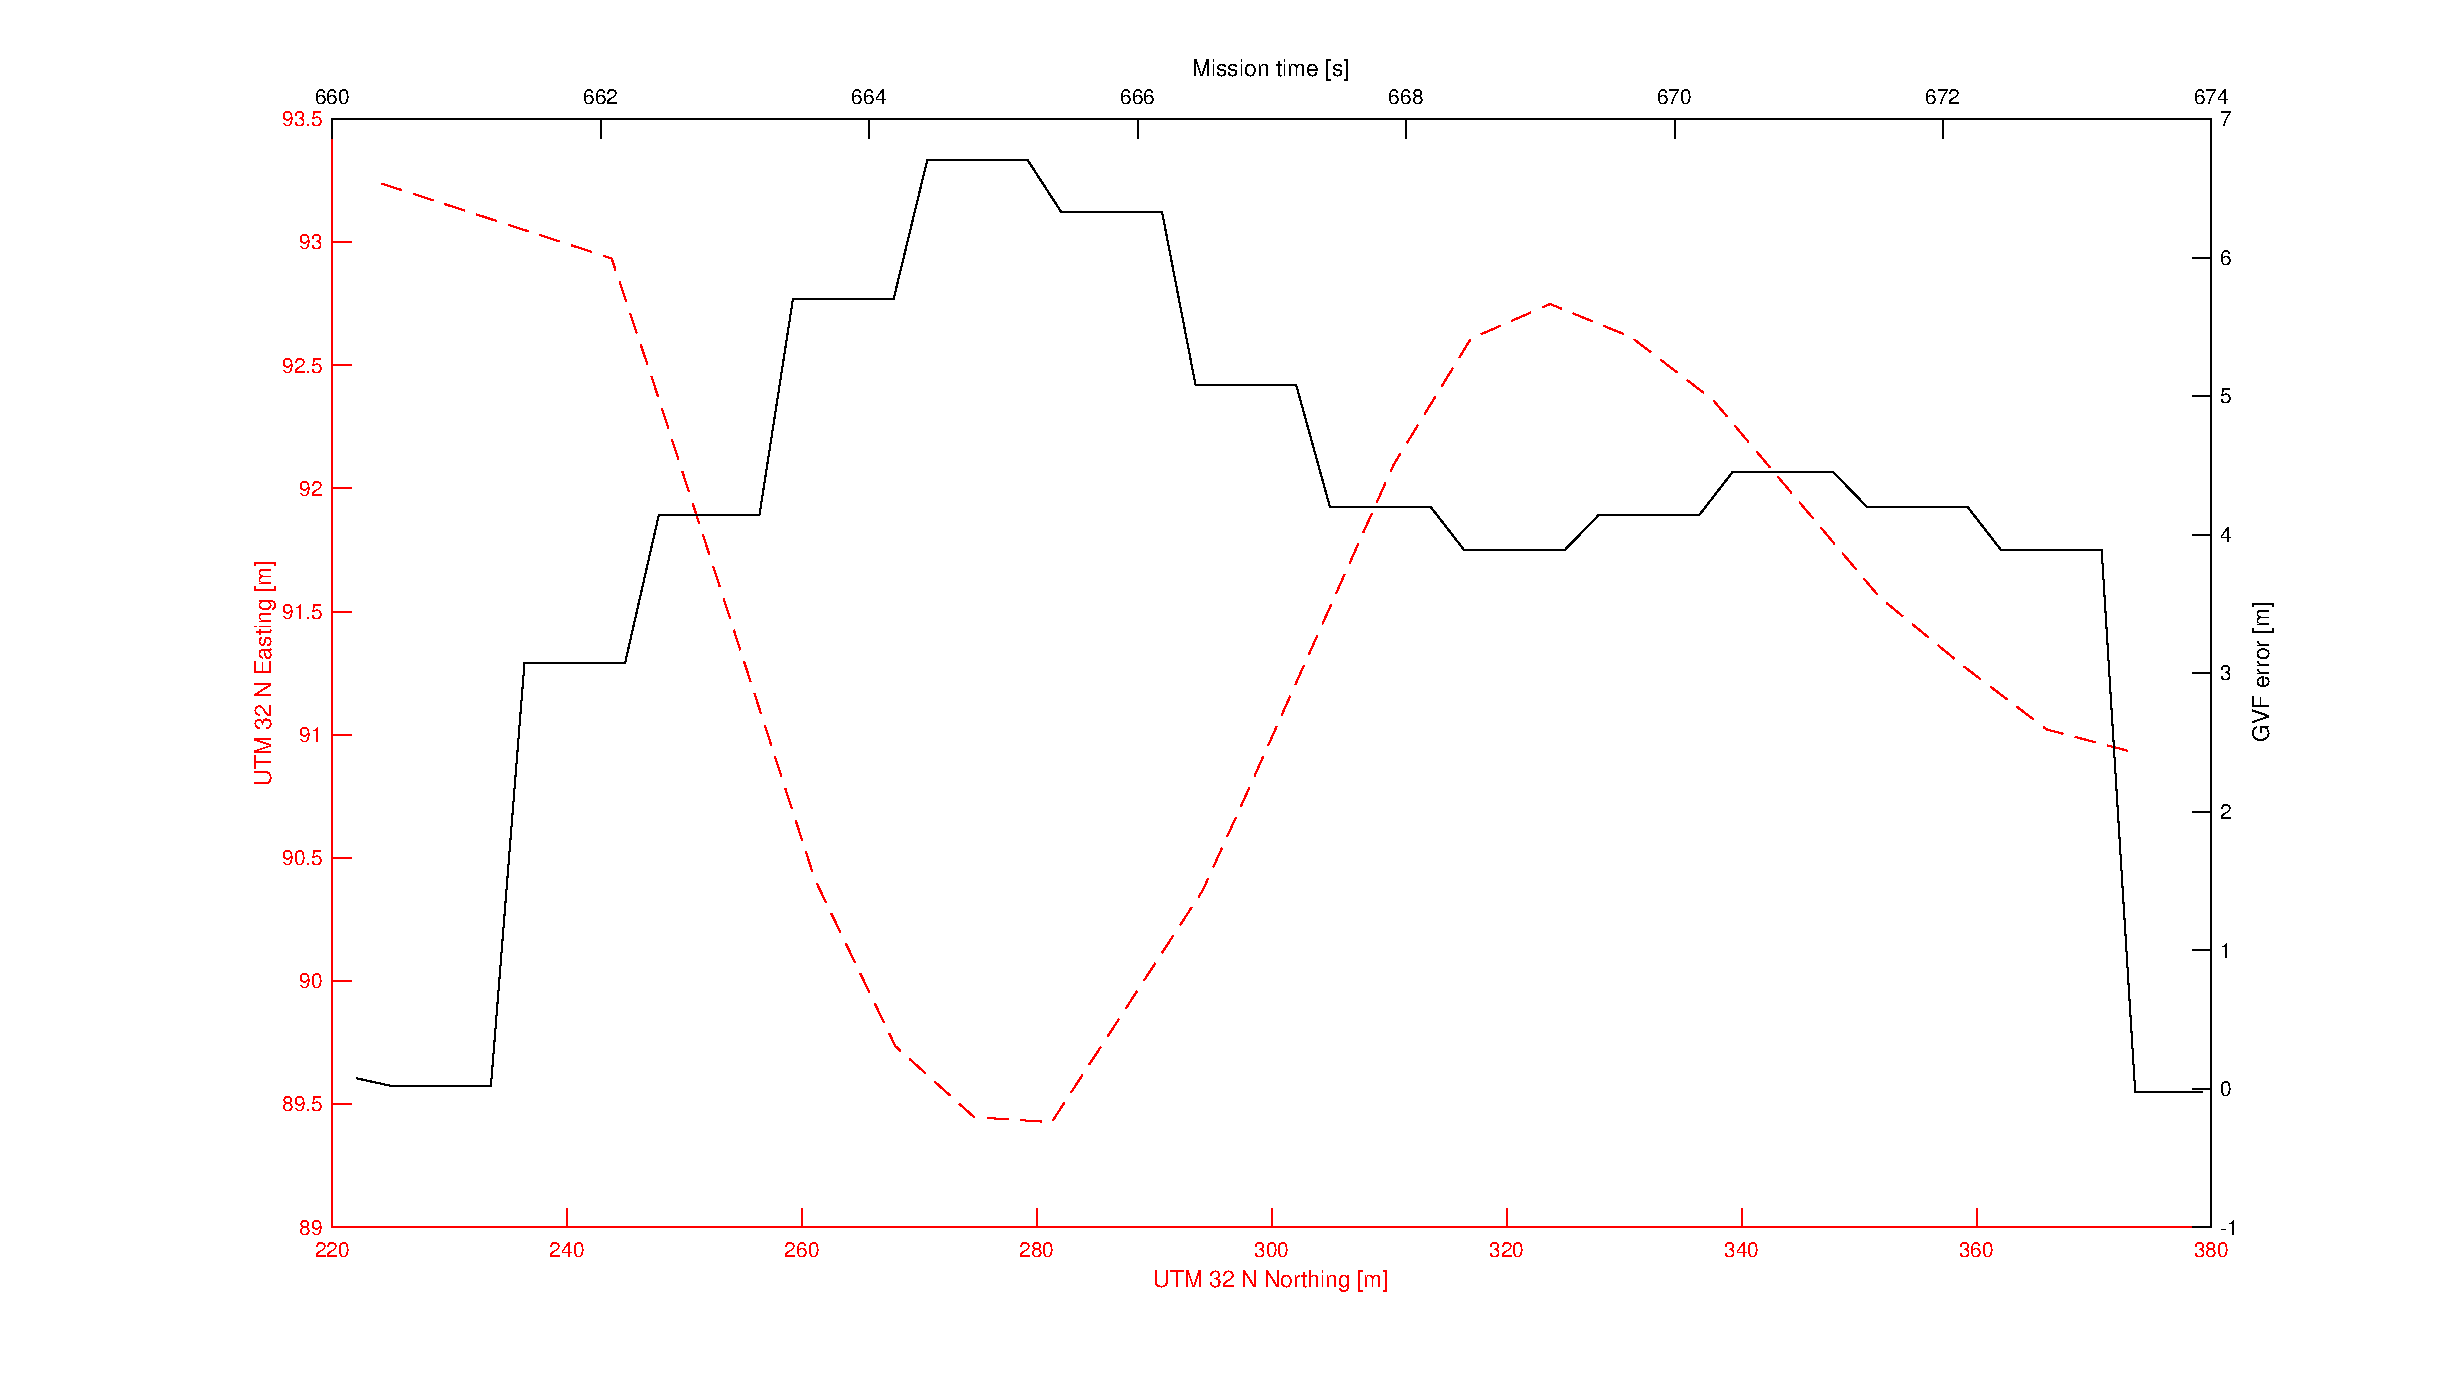
\includegraphics[width=16cm,height=16cm,keepaspectratio]{imagenes/graph.eps}
\caption{ Flight path line plot for surveying mission of field B}
\label{fig:FielB}
\end{figure}
\subsection{Front and side overlap}
When designing surveying mission flight path, two of the main criteria used are side and front overlap, these together with GSD are use to compute the distance between photos and distances between strips. These distances are the input for the navigation algorithm in charged of the navigation.
\subsubsection{Front overlap}
The front overlap is closely related to the distance between consecutive photos in the same path strip.  Using the geolocation of each photography is possible to find the distance traveled by the UAV between each picture. The spacing between the images should be 7.2 m, taking into consideration the error associated with GPS measurements of +- 4m. 

\begin{table}[H]
\centering
\begin{tabular}{|c|c|l|c|l|c|l|c|c|}
\hline
 & \multicolumn{8}{c|}{Number of photo in a X range of meters}                                                                                                                            \\ \hline
Surveying field         & \multicolumn{2}{c|}{X \textless 3.2} & \multicolumn{2}{c|}{3.2 \textless X \textgreater 11.2} & \multicolumn{2}{c|}{X \textgreater 11.2} & Turning points & Total                      \\ \hline
A                       & 6               & 5 \%               & 95                        & 81 \%                      & 17                 & 14\%                & 8              & 126                        \\ \hline
B                       & 3               & 2 \%                & 109                       & 79 \%                      & 26                 & 19\%                & 9              &  147 \\ \hline
\end{tabular}
\caption{Result of front overlap test}
\label{Table:FrontOverlap} 
\end{table}
\subsubsection{Side overlap}
The side overlap is closely related to the distance between of pictures on consecutive strips. plotting path flown by the UAV against the error signal of the GVF algorithm, it possible to determine the deviation  error in meters of the UAV trajectory to the designed trajectories. Figure \ref{fig:errorsignalGVF} show the before mentiond plot.
\begin{figure}[H]
\centering
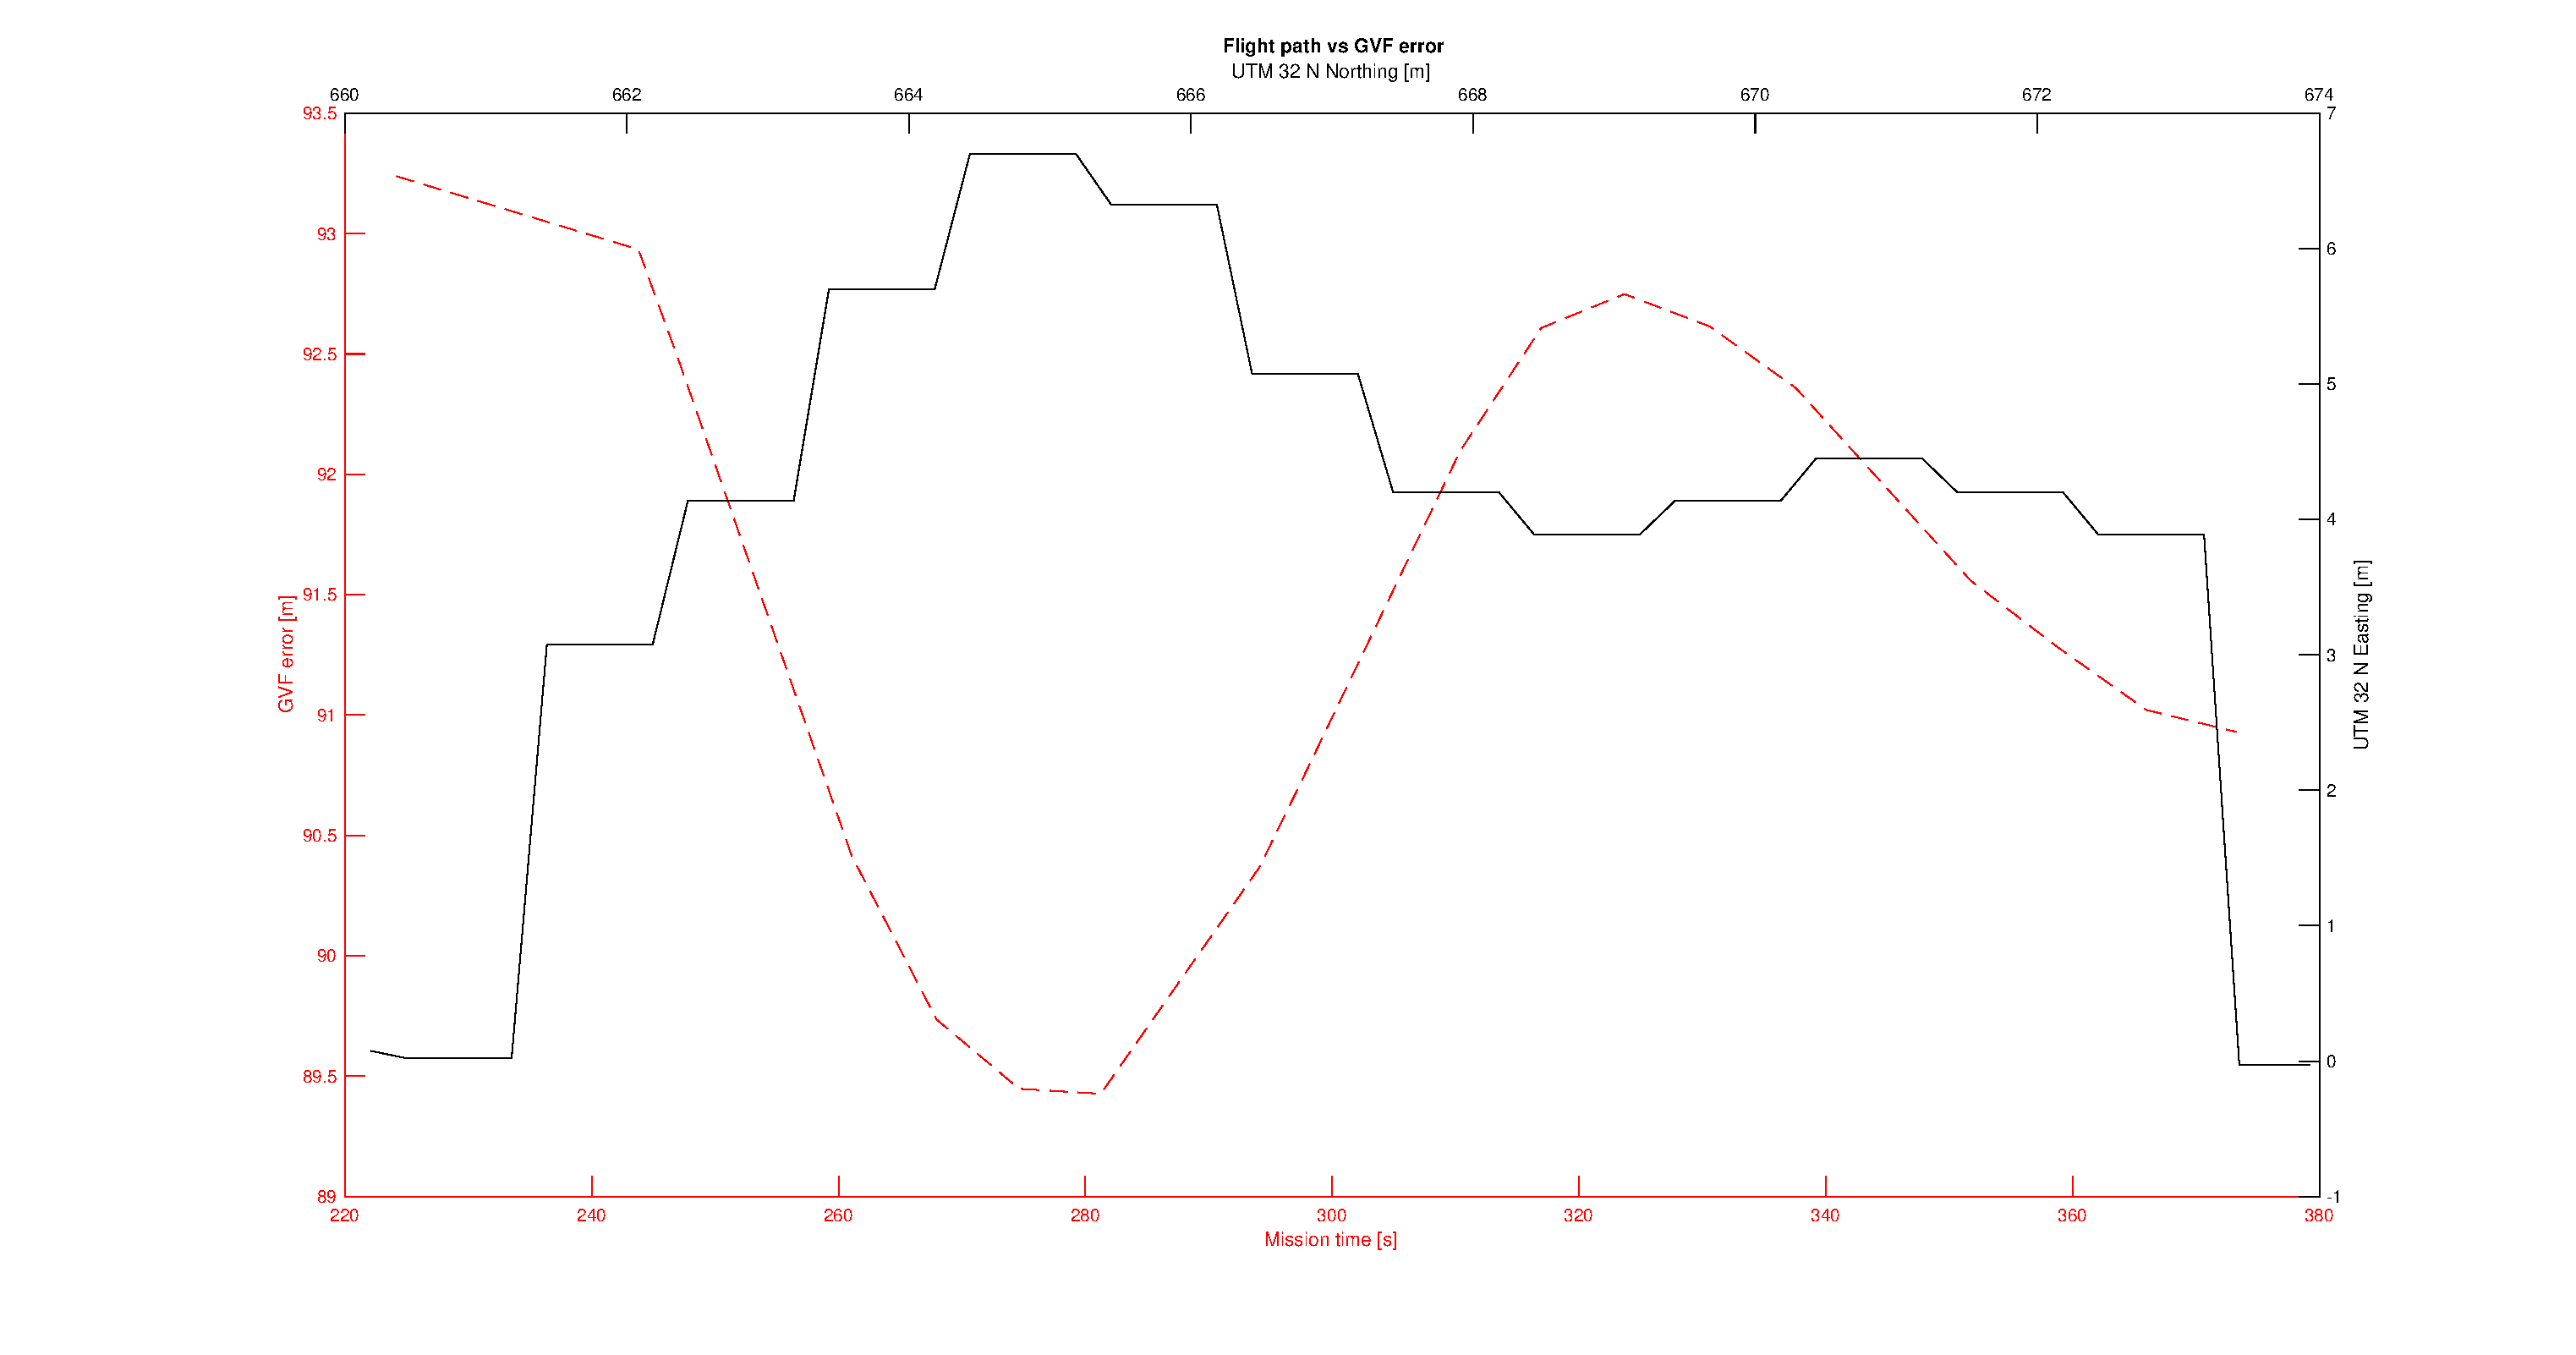
\includegraphics[width=16cm,height=16cm,keepaspectratio]{imagenes/StripvsGVF.eps}
\caption{Flight path vs GVF error}
\label{fig:errorsignalGVF}
\end{figure}
By analyzing the data of the GVF error signal during the surveying segment, it is possible to evaluate the accuracy of the trajectory of the UAV during the mission. Table \ref{Table:errorGVF} shows the GVF error signal trends during the surveying segments.
\begin{table}[H]
\centering
\begin{tabular}{|c|c|c|c|c|c|c|c|c|}
\hline
                & \multicolumn{8}{c|}{Flight strip number}               \\ \hline
Value           & 1    & 2    & 3    & 4    & 5    & 6     & 7    & 8    \\ \hline
Max {[}m{]}     & 6.70 & 5.80 & 5.53 & 5.63 & 4.80 & 5.71. & 9.00 & 7.52 \\ \hline
Average {[}m{]} & 3.78 & 3.15 & 3.18 & 2.22 & 2.58 & 3.02  & 3.84 & 3.50 \\ \hline
Media {[}m{]}   & 4.13 & 3.05 & 3.15 & 1.38 & 1.98 & 2.65  & 3.70 & 3.25 \\ \hline
\end{tabular}
\caption{GVF error analysis}
\label{Table:errorGVF}
\end{table}

\subsection{Photogrammetric products}
The image alignment, dense point cloud, and DEM construction were done using Agisoft Photo Scan Pro, and the results of the image processing procedure are shown in images \ref{fig:ResultBprocessing}, table \ref{Table:ResultsB} shown a more comprehensive data analysis of the different parameters of the mission.
\begin{figure}[H]
\centering
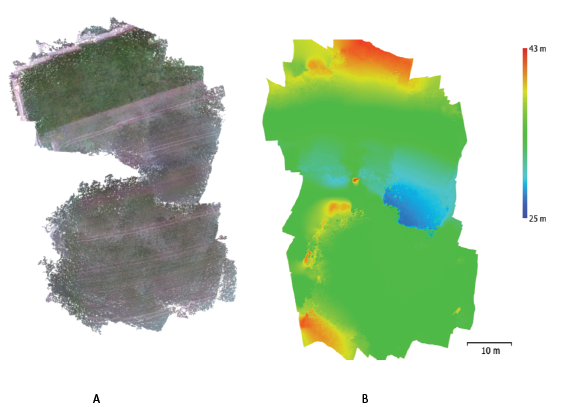
\includegraphics[width=16cm,height=16cm,keepaspectratio]{imagenes/ResutsB.png}
\caption{ A: Orthomosaic field B B: DEM field B}
\label{fig:ResultBprocessing}
\end{figure}

\begin{table}[H]
\centering
\begin{tabular}{|c|c|c|c|}
\hline
Surveying mission field B & Simulation & Experimental & Error (\%) \\ \hline
Fotos align               & -          & 147/147      & 0          \\ \hline
Altitude reported (m)     & 50         & 21.3         & 57.4       \\ \hline
GSD (cm/pixel)            & 1.33       & 3.5          & 62.2       \\ \hline
Coverage area (m2)        & 24000      & 7875         & 69.5       \\ \hline
\end{tabular}
\caption{Result of surveying mission over field B}
\label{Table:ResultsB}
\end{table}
Analyzing the data obtained from the software, is notable the error associated with the photogrammetric product are important. Although all the images were aligned, this process was not done correctly. Figure n shows an example of the error made by the alignment algorithm. 

There are several factors to take into consideration to explain the reasons for this behavior: the most important one: the Around 95 \% of pictures present \textit{vignetting}. Vignetting refers to the phenomenon of brightness attenuation away from the image center, and is an artifact that is prevalent in photography. Although not objectionable to the average viewer, it can significantly impair computer vision algorithms that rely on precise intensity data to analyze a scene. Applications in which vignetting distortions can be particularly damaging include photometric methods such as shape from shading, appearance-based techniques such as object recognition, and image mosaicing.  Figure \ref{fig:vignetting} shows a picture with vignetting.\cite{4663074}

\begin{figure}[H]
\centering
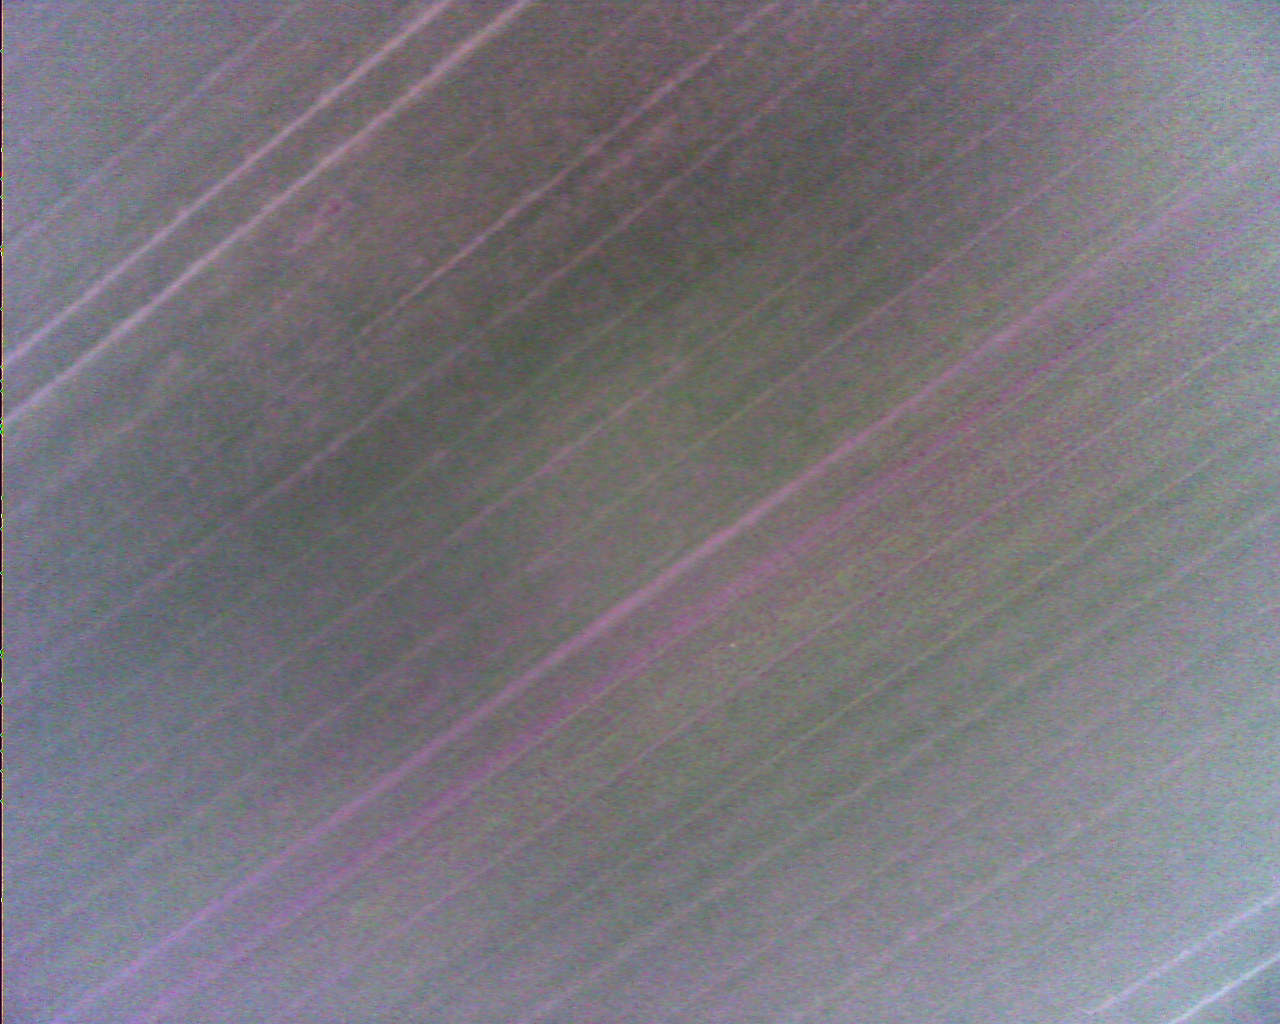
\includegraphics[width=16cm,height=16cm,keepaspectratio]{imagenes/IMG_62.png}
\caption{Picture with vignetting from the surveying mission}
\label{fig:vignetting}
\end{figure}
Table \ref{Talbe:XYerror} show the error of camera location estimator algorithm. taking into consideration that the field has a dimension of $X = 75 m and Y = 105 m$
\begin{table}[H]
\centering
\begin{tabular}{|c|c|c|}
\hline
   & \multicolumn{2}{c|}{Camera location estimation error} \\ \hline
   & Meters                     & \%                       \\ \hline
x  & 40.89                      & 45.3                     \\ \hline
Y  & 41.57                      & 60.3                     \\ \hline
XY & 58.31                      & --                       \\ \hline
\end{tabular}
\caption{Average camera location error}
\label{Talbe:XYerror}
\end{table}